\documentclass[11pt]{article}
\usepackage[english]{babel}
\usepackage[utf8x]{inputenc}
\usepackage{amsmath}
\usepackage{graphicx}
\usepackage[colorinlistoftodos]{todonotes}
\usepackage{indentfirst}
\usepackage{float}

\begin{document}

\begin{titlepage}

\newcommand{\HRule}{\rule{\linewidth}{0.5mm}} % Defines a new command for the horizontal lines, change thickness here

\center % Center everything on the page
 
%----------------------------------------------------------------------------------------
%	HEADING SECTIONS
%----------------------------------------------------------------------------------------


\includegraphics[scale=.2]{logo.png}\\[1.5cm]
\textsc{\LARGE Advanced Operating Systems}\\[0.5cm]
\textsc{\Large Written Report}\\[0.5cm]
MAB2 Computer Science\\
2017-18

%----------------------------------------------------------------------------------------
%	TITLE SECTION
%----------------------------------------------------------------------------------------

\HRule \\[0.4cm]
{ \huge \bfseries Sparrow: Distributed, Low Latency Scheduling}\\[0.4cm] % Title of your document
by Kay \textsc{Ousterhout}, Patrick \textsc{Wendell}, Matei \textsc{Zaharia}, Ion \textsc{Stoica}\\
University of California, Berkeley
\HRule \\[1.5cm]
 
%----------------------------------------------------------------------------------------
%	AUTHOR SECTION
%----------------------------------------------------------------------------------------

\begin{minipage}{0.4\textwidth}
\begin{flushleft} \large
\emph{Author:}\\
Arman \textsc{Davidyan}
\end{flushleft}
\end{minipage}
~
\begin{minipage}{0.4\textwidth}
\begin{flushright} \large
\emph{Supervisor:} \\
Dr. Alain \textsc{Buys}
\end{flushright}
\end{minipage}\\[2cm]

% If you don't want a supervisor, uncomment the two lines below and remove the section above
%\Large \emph{Author:}\\
%John \textsc{Smith}\\[3cm] % Your name

%----------------------------------------------------------------------------------------
%	DATE SECTION
%----------------------------------------------------------------------------------------

{\large \today}\\[2cm] % Date, change the \today to a set date if you want to be precise

%----------------------------------------------------------------------------------------
%	LOGO SECTION
%----------------------------------------------------------------------------------------

%
\includegraphics[scale=.25]{logo.png}\\[1cm]
 
%----------------------------------------------------------------------------------------

\vfill % Fill the rest of the page with whitespace

\end{titlepage}


\section{Introduction}


	Nowadays, the Internet services become more and more interactive: instantaneous language translations, highly personalized searches etc. This kind of jobs consist of many short, parallel tasks.\footnote{Note that every job is a set of tasks.} These kins of tasks, usually, have a duration around 100ms length. When each task is only around hundreds of milliseconds long, the cluster scheduler will need to work at very high throughput: a large cluster scheduler, treating this kind of tasks, will need to do over one million scheduling decisions. Usually, a cluster scheduler is a centralized application that keeps the state of the whole cluster and manages the task assignment to the worker machines. This architecture is more suitable for high-performance computing, but it can be difficult to support high throughput scheduling. This is the intention of Sparrow - a scheduler for low latency jobs.

    The first part of the report is an introduction to Sparrow. It will explain how Sparrow works and how well it performs in different scenarios. The second part of the job is a deepening in the subject of scheduling. It has two main topics: the first topic is an overview of the \textit{main architectures of cluster schedulers} and the second topic is a study of \textit{preemption} technique in the scheduling process. The report will end with a brief overview of the impact that Sparrow had on the industry.

\section{Sparrow}

	Sparrow is a cluster scheduler, dedicated to work with short, low latency tasks. It was introduced in the article \textit{Sparrow: Distributed, Low Latency Scheduling}, in 2013, by the searchers from University of California, Berkeley.


	\subsection{Architecture}
    	\label{sparrowarchie}

		The main idea of the Sparrow is having a scheduler that is decentralized. Sparrow is a set of scheduler that work independently (they do not exchange any information between each other). When a new job is submitted to the cluster, one these schedulers will get to assign its tasks to the worker machines. All of the schedulers work the same way - they are instances of the same simplistic scheduler. The exact way of assigning a job to a scheduler is not discusses in the article, but most probably it is done in round-robin manner.


	\subsection{Power of 2 choices}

		The set of schedulers that consist Sparrow are instances of the same simple scheduler. The main technique used in it, is called \textit{power of 2 choices}. This is a technique that came from article \textit{The Power of Two Choices in Randomized Load Balancing}, by Michael Mitzenmacher. \textit{Load balancing} is a problem of distributing $N$ tasks among $M$ resources, in the most even way. In the aforementioned work, M. Mitzenmacher proves that if instead of randomly choosing a resource for a task, we have a choice between two randomly chosen resources, the over-performance will be exponential.

		In some domains, this technique of chosen to random resources and assigning a task to the best suited one, could be a massive improvement over more complex techniques, because it has little overhead and can give good results. In \textit{Sparrow...}, the authors experiment to find out if this is still the case in the domain of cluster schedulers. But the power of 2 choices is not the only technique used in the scheduler - there are some others used to improve the overall performance.
        
        
    \subsection{Batch Sampling}
    
    	As it was stated, a job consist of some number of tasks, and power of 2 choices probes for each of this tasks individually two workers. This might not always return the best result. For example, if we have a job of two tasks, the probing for first task get return 2 workers with 3 and 4 pending tasks on them respectively, and the probing for second task can return workers with 1 and 2 pending tasks respectively. In this case the first task will be placed on the worker with 3 tasks and the second task will be placed in the worker with 1 task. But intuitively, it will be more efficient to place the first task on the worker with 2 pending tasks. This is exactly what \textit{Batch Sampling} does. When a job with $N$ tasks arrive, $2N$ random workers will be probed at the same time, and the tasks will be placed on the $N$ least loaded workers.


    \subsection{Late Binding}
    
    	There is one major flaw in the batch sampling and power of 2 choices in general - the number of pending task is not a good indicator of the business of the worker. If we have two workers, one with 4 pending task and another with 1 pending task\footnote{both workers are single core}, it does not always mean that it is better to place the new task on the worker with one task. If each of the 4 task will take 10 ms and the the single task on the other worker takes 200 ms, then the first worker will be available to execute a task sooner. This is why many cluster schedulers \textit{Late binding}. This is a technique that places reservations on $2N$ random workers for a job with $N$ tasks, instead of placing the task right away. When a worker is available to execute the task, it will notify the scheduler that placed the reservation and the latter will send the task to the worker. This way, the tasks are assigned to the workers that are available first. When all the task are assigned to fastest $N$ workers, the other $N$ workers will get a message to forget about the reservations.


    \subsection{Experiments}
    
    	To test the efficiency of Sparrow, the authors performed some number of tests. Some of tests are completely analytic, which means no tests on hardware were done, and some are practical. Among practical experiments, they did 2 kind of test: with real world workloads and with synthetic workloads. All the practical experiments have been performed on a cluster of 110 machines. To perform the experiments, Sparrow was integrated in the Apache Spark cluster framework (it replaced Spark's native scheduler).


		\subsubsection*{Theoretical Analysis}
        
        	The authors did only one theoretical study of Sparrow. The point of this study was to discover the probability for a job to experience a zero wait time \textit{i.e.} the probability for all task of a job to be placed on idle machines.
            
            \begin{figure}[H]
            	\centering
                \begin{tabular}{ | l | l |}
                    \hline
                    Random Placement & $(1-\rho)^m$  \\ \hline
                    Power of 2 choices & $(1-\rho^d)^m$  \\ \hline
                    Sparrow & $\sum_{i=m}^{d*m}(1-\rho)^i$$\rho^{d*m-i}$${d*m}\choose{i}$ \\
                    \hline
                \end{tabular}
                \caption{$\rho$ is the cluster load, $d$ is probe ration and m is the number of tasks in a job.}
        	\end{figure}
            
            In the table above one can see the probabilities for 3 different techniques to place all tasks of some job on idle workers, in a cluster with single core machines. The authors varied the cluster load from 0 to 1 and fixed the probing ratio of 2 to obtain a graph that showed that the theoretical probability of Sparrow to place all task on idle machines is very close to 1 when the cluster load is lower then 0.5 and it is very close to 0 when it is higher than 0.5.
            
            The authors also performed the same test on a cluster with 4 core machines. They added an additional constrains to avoid ``gold rush effect'': because of the fact the decentralized schedulers in Sparrow does not share any information between each other, if two of them find the same idle worker at the same time, both will place 4 tasks on that worker; hence, there will be 4 tasks that will experience an unexpected delay. To avoid this problem, Sparrow let each scheduler to place only one task on a worker. The result of this experiment is that 79.9\% of jobs will be placed on idle worker at 80\% workload.
            
            
        \subsubsection*{Experiment with TPC-H queries}
        
        	Another experiment that authors performed was executing queries of TPC-H benchmark on a cluster scheduled by Sparrow. TPC-H\footnote{TPC-H stands for Transaction Processing Council Ad-hoc/decision support benchmark} is a benchmark frequently used for testing the performances of database softwares. It contains sets of queries that are inspired from real-world scenarios.
            
            The authors composed 4 different sets of queries: first set keeps the cluster load at 80\%, the second set contains the queries that have two groups of tasks that can not be processed in parallel, the third set contains the queries with task that have mixed durations, and the forth contains the queries with tasks that have different constraints.
            
            The result of this experiment showed that, in average, Sparrow performed only 12\% worse than the ideal scheduler. The performance of the ideal scheduler was computed by supposing that it always placed tasks on idle workers (no task was queued, no job experienced any waiting time). In other words, the execution time of a job, scheduled with the ideal scheduler, is equal to the longest, non parallel sequence of tasks in it.
        
        
        \subsubsection*{Experiment with a scheduler's fail}
        
        	Sparrow is contains some number of simplistic scheduler and all of them can fail. In the case of a failure, it is necessary to be sure that the jobs assigned to the failed scheduler are still executed. For this purpose, each of the scheduler is launched with a list of backup schedulers, and Sparrow verifies every 100 ms that they are functional. If one of the scheduler fail, Sparrow will assign the jobs that were currently pending to the first scheduler in the backup list (of the failed scheduler). The intermediate progress of a job acquired before the failure will be lost. An experiment showed that the job that Sparrow relaunches a failed scheduler in 120ms from the moment of its fail. Because of the fact that the Sparrow is dealing with short tasks, only few jobs will be penalized because of a scheduler's failure.
        
        
        \subsubsection*{Sparrow compared to a centralized scheduler}
        
        	In a case of centralized scheduler, all the scheduling decisions are made by a single agent. Because of it, this king of schedulers are more convenient for High-Performance Computing. To prove that, the authors compared the performance of Sparrow with the performance of Sparks native centralized scheduler on a cluster at 80\% workload. The experiment showed that when the duration of the tasks are 1.3 second or less, the Spark's native scheduler is no longer able work properly and experience infinite queuing.
        
        
        \subsubsection*{Sharing a cluster between multiple users}
        
        	To analyze how fairly Sparrow is capable to share a cluster between many different user, the authors performed an experiment with a cluster shared between two users. The first user always requires as much resources as possible from Sparrow all the time during the experiment. The second user requires no resources at all for ten seconds; then he requires 25\% of the cluster capacities for another 10 second; then he requires 50\% of the cluster capacities for another 10 seconds; then he requires only 25\% of the capacities for another 10 seconds; for the last 10 second interval, the second user requires no resources at all.
            
            The result of this experiment showed that Sparrow is able to fairly share the cluster between different user, but sometimes the cluster may be used not at the maximum of its capacities. The reason of this problem is related of the decentralized nature of Sparrow - it contains many scheduler that are not inter-connected, hence, they don't have the complete image of the cluster utilization by user.
        
        
        \subsubsection*{Shielding high priority tasks users from low priority users}
        	 \label{preemption}
        	
            An important aspect of a Sparrow is protecting users high priority user from low priority users. To do so, the authors implemented Sparrow in the following way: each worker has many queues - each of them contains only tasks with the same priority and no node has two queue with the tasks of the same priority. When a worker has completed a task, we will pull a task from the highest non-empty queue.
            
            In this experiment, the authors kept the proportion of the high priority load at 25\% of the cluster capacities and varied the proportion of low priority load. The experiment showed that Sparrow is able to protect the high priority tasks from low priority task when the total cluster load is less than 100\%. But, when the total cluster  load is at 100\% or more, the high priority get 40\% worse execution time.
        
        
        \subsubsection*{Why power of 2}
        
        	Another interesting point for authors was to find out if the probing ratio of 2 is the best choice or it is better to have a higher of lower probing ratio. To answer to that question, the authors performed two experiments where they varies the probing ratio, but kept constant the cluster load. The first experiment kept the cluster load at 80\% and the second one kept it at 90\%. The range of probing ratio was between 1.0 (random placement) to 3 (3 probings par task). The experiments showed that the best probing ratios are 1.5 and 2, because if the probing ratio is lower, the schedulers are not able to find idle workers, and if the probing ratio is higher, there is too much message exchange in the cluster and that also delays the probing decision. The authors choose the probing ratio of 2 because it is easier to have an integral probing ratio.


\section{Main architecture of cluster scheduling}

	The authors of Sparrow adapted a specific architecture for the process of scheduling tasks. To better understand the choices they made during implementing Sparrow, it will be useful to take a look at mainstream cluster scheduler.
    
    %NOTE remove the explanation of schedulers?
	Every major company adapts its cluster scheduler to its needs, but basically, one can divide them in three large categories: monolithic, two-level and shared state. Monolithic schedulers are the most populars. A scheduler of this type is using a centralized algorithm for all jobs. For example, Borg, created and used at Google, is a monolithic scheduler. Two-level schedulers have a single resource manager and many parallel scheduling (like Sparrow). The parallel schedulers are not necessarily homogeneous, and the single resource manager share the resources between them. Mesos \cite{mesos} is an example of these kind of scheduler. In the case of shared state schedulers, there are many parallel, not necessarily homogeneous, schedulers. Each of the schedulers has a complete view of the cluster load, and there are no direct interactions between schedulers. Omega \cite{omega} is an example of shared state cluster. The architecture of shared state clusters is the closest, among the 3 aforementioned architectures, to the architecture of Sparrow. Figure 1 illustrates an overview of the three architectures.
    
    \begin{figure}
    	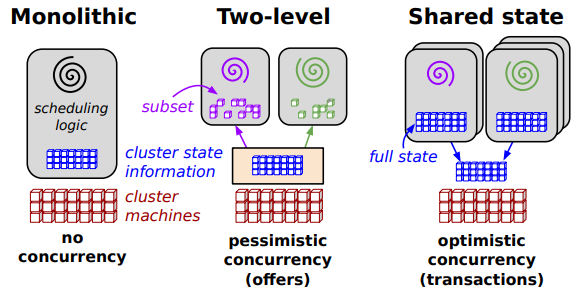
\includegraphics[scale=.6]{architectures}
        \caption{An overview of the most popular scheduling architectures. The source of this figure is \cite{omega}. Because of the fact that \cite{omega} discusses only monolithic, two-level and shared states scheduling techniques, the fully-distributed and hybrid scheduling techniques are not illustrated.}
    \end{figure}

	\subsection{Monolithic scheduling}
    
    	%TODO add Borg
    	As it was stated above, the monolithic schedulers are the most popular cluster schedulers. They have a central agent that performs all scheduling decisions and sees the cluster resources as a single entity. This approach is most suited for high-performance computing because in HPC we worry less about the speed of execution then in modern clusters. Usually, the centralized agent is a complicated algorithm because it must contain all the policies and constrains of the system. Also, the scheduling algorithm gets updated over time which leads to a very complicated code base, and a difficulties to future updates. But the most dangerous situation that can be faced with a monolithic scheduler is the side effects. When the code gets complicated, a lot of undocumented side effects appear, and the developers tends to use them in order to optimize their programs. The problem is that once the code of the scheduler is changed, some side effects can disappear and the programs using them will no longer work.
        
        Usually, the central agent contains does all the necessary functions to compute the priority of a task. After the priority is computed, all tasks are ordered by their priority and the execution will start by the tasks in the head of the list. Some schedulers support code paths with the jobs. In this case, the actor that submits the job can also submit a path to a code that the scheduler will execute in order to find the priority of a task. In this way, the standard policies of the scheduler can be overridden for certain jobs.
        
       %NOTE add statically partitioned schedulers
       
	\subsection{Two-level scheduling}
    
    	This type of scheduling was first introduced by Mesos \cite{mesos}. Two-level schedulers have a single resource manager, but many scheduling frameworks. The purpose of the resource manager is dynamically defining the resources for each scheduler. The manager offers to the scheduler only the resources that are currently unused, and any resource is offered only to one scheduling framework at a time, to avoid conflicts. An important goal of the resource manager is to share the resources fairly between frameworks. YARN [cite], another two-level scheduler used in Apache Hadoop\footnote{Hadoop is an open-source framework that allows processing large data sets across cluster of computers}, lets the scheduling frameworks to ask from resource manager the resources it needs, instead of waiting for an offer.
        
        The scheduling frameworks in the two level schedulers can be heterogeneous. This means that each framework can target only some particular type of jobs. This distinction between different frameworks can be based on task durations, parallelism of tasks in a job, some constrains of the job etc. The scheduling frameworks have only access to a part of the cluster and do not see the state of whole cluster. Because of this fact, the gang scheduling (more on this in [ref]) might be difficult to implement (because some tasks can require different different types of resources, and all the tasks must be executed at once). Some schedulers as Mesos \cite{mesos}, can let its scheduling frameworks to accumulate resources needed for a gang scheduling, but this might lead to deadlocks.
    
    \subsection{Shared state scheduling}

		A shared state scheduler contains many scheduling frameworks, but no resource manager. The frameworks can be heterogeneous and need to compete with each other to obtain a resource. Each framework contains an replica of the cluster state. If one framework wants to request some resource, it should update its local replica and will send the information about the request to other frameworks. The request may fail if another framework requests the same resource in the meantime. Usually, the scheduling is done in incremental manner - a framework occupies all non-conflicting resources. Although, to perform gang scheduling (all task executed at the same time, or none), a framework can do atomic request - all resources or nothing. Examples of his king of scheduling are Omega \cite{omega} by Google and Apollo \cite{apollo} by Microsoft.
    
    \subsection{Fully-distributed scheduling}
    	%TODO has distributed scheduling gain any popularity?
    	This kind of scheduling is similar to shared state scheduling, except that the scheduling frameworks don't interact between each other. The schedulers compete with each other to obtain the resources. As Sparrow is an example of a fully-distributed scheduler, a more detailed explanation of this kind of scheduling can be found in \ref{sparrowarchie}.%TODO talk about the disadvantages of fully-distributed scheduling?
        
    \subsection{Hybrid scheduling}
    
    	A hybrid scheduler adapts two or more techniques at once. For example, we can combine the techniques of monolithic scheduling and fully-distributed scheduling. A hybrid of this kind should have a central algorithm that decides how a job should be scheduled; if the tasks are short and can be executed in parallel, the job can be scheduled under fully-distributed scheduling technique, otherwise it should be scheduled by the monolithic scheduler.


\section{Possible improuvements}

	Sparrow is very simplistic cluster scheduler - the only techniques it adapats are power of 2 choices, batch sampling, late binding and proactive cancelation. The authors of Sparrow realized that, and during the work, they mentioned on multiple occasions that it needs improuvements. They even provided a list of techniques \cite[section 8]{sparrow} that are used in different schedulers and can improuve Sparrow. Unfortanantly, they were brief in explanation. It would be useful to dig depper in this subject to see what are these techniques, and understand if they are possible to implement in Sparrow.
	
	\subsection{Preemptive scheduling}
	
		Preemption is the process of interrupting a task that is currently executing, in favor of a new task with higher priority that has just arrived. Preemptive scheduling is one technique that is implemented for most of the schedulers, but for Sparrow. In \cite[subsection 7.8]{sparrow}, also explained in \ref{preemption}, the authors studied the effect of low prioirty tasks that are abusing the resources of cluster and not letting the task with high prioirty task to be executed in time. In the experiment, only 25\% of the cluster load was high priority tasks, hence, they could be, and they should be, executed in time. But, because of overpressure of low priority tasks, they get 40 \% worse execution time in average. If Sparrow had preemption, the shedulers could have interupted some low prioirty tasks in favor of high prioirty tasks, and the important job would have shorter execution times.
		
		Preemtion scheduling seems to be fairly easy to implement in Sparrow. For recall, Sparrow keeps $N$ priority queues on each working machines; rach of these queues is dedicated to tasks to only one level; when a new slot is empty, the worker is going to take the first reservation from the highes priority queue. If we implement preemption in Sparrow, then, each time a worker gets a new reservation, it should verify if the task in execution (or one of tasks in the execution) has lower priority than the new task.
		
		The only problem related to preemption is context swithching. When a task is preemted, its current state and variables are stored locally, until the execution can be resumed. The problem Sparrow can face is the rightfullness of the context switching. It is possible that is some scenarios (for example when current task is extreamly short or very close to its end), the context switching will take more time than waiting for the current task to end. It is an important problem because Sparrow is a scheduler for short, low latency tasks. Also, after implementing the preemption scheduling, additional experiments should be made (and some experiment should be redone), to understant how the preemption affected the overall performance of Sparrow. It is possible that it will worsen the avarage task duration. If it is the case, the authors should make a choice between preemption and overall performance.
		
		
		%The preemption should be done by the workers, not by the scheduling frameworks, because the shedulers do not know anything about the tasks that are currenty pending on worker, they only get notified when a worker is redy to execute it tasks. But, we can't wait until a worker notifies the scheduler with high priority task. Hence, we implementaton of Sparrow should be change in a way that the scheduling frameworks will send to workers the imformation about the priority of task thay want to schedule. When a worker resives a probing from a scheduler, it would verify if scheduler's task has higher priority than the currently executing task (or one of currently executing tasks). This will complicate the software of working machines because, currently, it is very simplistic - if there is a free slot, a new task with the higer
		
			
		




\begin{thebibliography}{9}

\bibitem{sparrow}
  K. Ousterhout, P. Wendell, M. Zaharia, I. Stoica,
  \textit{Sparrow: Distributed, Low Latency Scheduling},
  SOSP '13,
  Pages 69-84 ,
  Farminton, Pennsylvania,
  November 03 - 06,
  2013.

\bibitem{omega}
  M. Schwarzkopf, A. Konwinski, M. Abd-El-Malek, J. Wilkes,
  \textit{Sparrow: Distributed, Low Latency Scheduling},
  EuroSys '13,
  Pages 351-364,
  Prague, Czech Republic,
  April 15 - 17,
  2013.
  
\bibitem{mesos}
  B. Hindman, A. Konwinski, M. Zaharia, A. Ghodsi, A. D. Joseph, Randy Katz, Scott Shenker, I. Stoica,
  \textit{Mesos: A Platform for Fine-Grained Resource Sharing in the Data Center},
  NSDI'11,
  Pages 295-308,
  Boston, Massachusetts,
  March 30 - April 01,
  2011.
  
\bibitem{borg}
  A. Verma, L. Pedrosa, M. Korupolu,
  \textit{Large-scale cluster management at Google with Borg},
  EuroSys '15,
  Article No. 18,
  Bordeaux, France,
  April 21 - 24,
  2015.

\bibitem{apollo}
  E. Boutin, J. Ekanayake, W. Lin, B. Shi, J. Zhou, Z. Qian, M. Wu, L. Zho,
  \textit{Apollo: Scalable and Coordinated Scheduling for Cloud-Scale Computing},
  OSDI' 14,
  Pages 285-300,
  Broomfield, Colorado,
  October 6 - 8,
  2014.

\end{thebibliography}

\end{document}



























